\documentclass[11pt,twocolumn]{article}
\usepackage[margin=0.8in]{geometry}                % See geometry.pdf to learn the layout options. There are lots.
\geometry{letterpaper}                   % ... or a4paper or a5paper or ... 
%\geometry{landscape}                % Activate for for rotated page geometry
%\usepackage[parfill]{parskip}    % Activate to begin paragraphs with an empty line rather than an indent
\usepackage[breaklinks=true, colorlinks=true, linkcolor=red, urlcolor=blue, citecolor=black]{hyperref}
\urlstyle{rm}
\usepackage{amsmath}
\usepackage{mathptmx}
\usepackage{graphicx}
\usepackage{amssymb}
\usepackage{epstopdf}
\usepackage{color}
\usepackage{sidecap}
\usepackage{authblk}
\usepackage{booktabs}
\usepackage[font=small,labelfont=bf]{caption}
\DeclareGraphicsRule{.tif}{png}{.png}{`convert #1 `dirname #1`/`basename #1 .tif`.png}
\usepackage{enumitem}
\setlist[itemize]{noitemsep}
\setlist[enumerate]{noitemsep}

\def\bfr{\bf\color{red}}
\def\geohub{{\tt geohub}}
\def\Count{count}
\def\ntracts{39}
\def\nprof{9}
\def\nvol{30}
\def\resp{respectively}

\title{\bf
	Results of the 2021 Volunteer Homeless Count in Hollywood
	}
\author[1,$\ast$,$\dagger$]{Louis Abramson, PhD}%,$\ddagger$
\author[2]{Brian Kohan}%,$\ddagger$
%\author[1]{Kerry Morrison}%,$\ddagger$
%\author[2]{Jackie Vorhauer}%,$\ddagger$
\affil[1]{\it \small Hollywood 4WRD Homelessness Coalition, 6255 Sunset Blvd, Ste 150, LA, CA 90028}
\affil[$\ast$]{\it Central Hollywood Neighborhood Council, PO Box 93907, LA, CA 90093}
\affil[$\dagger$]{\it Carnegie Observatories, 813 Santa Barbara St, Pasadena, CA 91101}
\affil[ ]{\href{mailto:labramson@carnegiescience.edu}{labramson@carnegiescience.edu}}

\date{\today}                                           % Activate to display a given date or no date

\begin{document}
\maketitle

\begin{abstract}

%The Los Angeles Homelessness Services Authority (LAHSA) opted not to sponsor a 2021 Unsheltered 
%Point In Time Count. Despite this, service providers, business leaders, residents, and other organizations
%in Hollywood decided to proceed with an analogous if unsponsored event on 25 February 2021. XXX 
%volunteer vehicle-based teams and YYY professional foot outreach teams performed visual inspections of
%all 39 US Census tracts in the official Hollywood and East Hollywood Continua of Care (CoCs). Based on 
%the 2020 official LAHSA dwelling weighting factors, we estimate that there are $xxx\pm yyy$ unsheltered 
%people living on the streets of those CoCs (90\% confidence). Modulating the weights leads to variability
%of XXX. We conclude that YYY. All data and results are presented in tabular form, with materials, and
%analysis code presented in the Appendix or on request.

\end{abstract}

\section{Introduction}
\label{sec:intro}

The Los Angeles Homelessness Services Authority (LAHSA) typically conducts a Point In Time (PIT) 
census of the unhoused population of Los Angeles County annually. These data inform programmatic
funding levels, educate residents, undergird local and state legislative efforts, and shape the day-to-day 
practices of thousands of professional and volunteer service providers. As the official assessment of the 
scope of one of the most pressing humanitarian issues of our time, the LAHSA Count is invaluable.
However, due to disruptions from COVID-19, LAHSA decided to cancel the unsheltered portion
of the 2021 PIT count. As roughly 70\% of LA's unhoused residents are unsheltered, this move ensures
data on homelessness immediately following one year of unprecedented economic disruptions and
government interventions will be substantially incomplete.

Greater Hollywood is an epicenter of LA's homelessness crisis. According to the official 2020 
Count, the Hollywood and East Hollywood Communities were home to 2203 unhoused residents,
1714 of whom (78\%) were unsheltered. This figure corresponds to roughly 5\% of LA's homeless 
population concentrated in an area with only 2.5\% ({\bfr CITE}) of its total population. In some 
regions in those communities, 1-in-30 residents are unhoused compared to 1-in-100 citywide.

\begin{figure*}
	\centering
	\includegraphics[width=0.9\linewidth]{countMap}
	\caption{The 2021 volunteer \Count\ covered Greater Hollywood, comprising the 
			officially recognized LAHSA Hollywood and East Hollywood Continua
			of Care. The former stretches from Laurel Canyon Blvd to Western Ave,
			the latter from Western to Hoover Ave. Hollywood is bounded to the north
			and south respectively by Franklin	and Melrose Aves, with East Hollywood
			bounded by Hollywood Blvd and Beverly Ave. Hollywood comprises
			21 census tracts; East Hollywood 18. The grey lines above show census 
			sub-tracts used by LAHSA but ignored in this \Count.}
	\label{fig:map}	
\end{figure*}

While the above statistics are tragic, Hollywood is also marked by increasingly formal coalitions of 
service providers, business leaders, residents, and quasi-governmental entities dedicated to humanely 
ending the homelessness crisis. Each of these stakeholders relies on the annual PIT count: lay residents need
to be educated as to the size of the challenge; funders need to understand how many people require services;
legislators need to know how many people are dwelling where. For these reasons, and given the 
capacity of the above organizations and individuals, the Hollywood community decided to proceed with 
an unsponsored 2021 grassroots PIT \Count.

This document describes the methodology and findings of that \Count, which took place on Thursday, 
February 25, 2021. Section \ref{sec:procedure} describes data acquisition, analysis, and volunteer
training protocols. Section \ref{sec:results} present estimates of the unsheltered 
populations in the Hollywood and East Hollywood CoCs and contextualizes those findings in terms of 
previous LAHSA results. Section \ref{sec:systematics} describes factors that would
modulate them up or down. Section \ref{sec:summary} summarizes. Additional information
can be found in the Appendix, including a table of tract-level results in each of the survey's 39 US 
Census tracts.

\section{Methodology}
\label{sec:procedure}

Our \Count\ took place on 25 February 2021, with the majority of census tracts surveyed beginning
at 7.00 PM. This timing corresponds to one month later and four hours earlier than the official event 
would have occurred. Beyond those choices, our program adhered as closely as possible to the official 
LAHSA 2020 PIT data collection and analysis protocols. Ancillary data from regularly monitored 
census tracts suggests that the date offset is unlikely to substantially erode comparability between 
this and past datasets. Limited daytime recounts also suggest that time-of-day effects are sub-dominant.

The \Count\ was based out of The Center at Blessed Sacrament (``The Center''), a major service 
provider in Hollywood, at 6636 Selma Ave. All volunteer teams launched from and returned to this 
location as they would in previous years to a LAHSA community count hub. The major difference 
was that training was performed remotely as a COVID precaution and volunteer counters never left 
their vehicles.

\subsection{Data Acquisition}
\label{sec:acquisition}

The \Count\ covered the \ntracts\ US Census tracts constituting the LAHSA-defined Hollywood 
and East Hollywood Communities (21 and 18 tracts, \resp). Our \Count\ did not recognize census 
tract ``splits'' or sub-tracts---e.g., ``1905.10a''---which sets a coarser resolution floor to our results 
compared to past PIT results. That choice also slightly modifies of the definition of both communities:
Hollywood includes all of tract 1905.10 as opposed to only the ``a'' sub-tract, and East Hollywood
includes all of 1913.01 instead of just the ``b'' sub-tract. Such modifications have an insignificant impact 
on community-level results---since 2016, 1905.10b has never been seen to host more than 7 
unsheltered people; 1913.01a never more than 15. Sections \ref{sec:results} and \ref{sec:discussion} 
discuss community-level results with tract-level tallies provided in the Appendix. Results for Greater 
Hollywood are not directly comparable to any official service geography but are available upon request. 
Figure \ref{fig:map} shows the \Count\ footprint.

All tracts were vetted by professionals from The Center prior to assignment. Tracts deemed 
especially challenging---due, e.g., to their proximity to freeway onramps and peripheries---were 
reserved for professional counting teams. Vetting produced \nprof\ such tracts, which were surveyed 
by outreach personnel from The Center and Covenant House---another local provider---circa 3:00 PM
on 25 February. The remaining \nvol\ tracts were divided among the volunteer vehicle-based teams 
and surveyed beginning at 7.00 PM. Importantly, with the exception of one tract in East Hollywood, 
teams were restricted to one or the other community, making the community-level results nearly
independent. Cross-comparisons therefore serve as data quality indicators (Section \ref{sec:discussion}). 
Table \ref{tbl:tractStats} records which tract was counted by which kind of team. 

Thirty-two volunteer vehicle-based teams participated in the \Count\ itself, which was limited to 
existing COVID ``pods'' of two to three people to ensure that the possibility of transmission minimized. 
Singlet volunteers were admitted but remained on-site to assist with traffic control and material distribution. 
All participants wore personal protective equipment and maintained social distancing when appropriate.

Counting followed 2020 LAHSA PIT protocols to the greatest extent possible. Each vehicle-based 
volunteer team comprised at least a Driver and a Counter and was assigned two tracts to count. 
Three-person teams also included a Navigator. In such teams, the Navigator directed the Driver while 
the Counter tallied unhoused individuals/dwellings. In two-person teams, the Counter doubled as 
the Navigator. Training emphasized techniques aimed at reducing the Counters' cognitive loads and 
so minimize counting errors. These included driving slowly using hazard lights and covering interior 
streets in a serpentine pattern before circling the tract border. Teams were instructed to count both 
sides of interior streets but only interior sides of border streets. Teams were also instructed to watch
the official training video from the 2020 PIT count in addition to receiving the training from our
team.

Upon arriving at The Center, organizers gave each team a clipboard with:
\begin{itemize}
	\item tract maps (2$\times$);
	\item tally sheets (2$\times$);
	\item a 1-page training summary with a contact number for in-field issues.
\end{itemize}
Examples of each of the above documents are included in the Appendix. The latter was used 
once to alert site volunteers to the possibility of an unaccompanied minor.

The tally sheets---the data acquisition tool---contained separate columns for each of the nine 
categories of unhoused individuals or dwellings recognized in the 2020 LAHSA PIT count: 
\begin{enumerate}
	\item adults (ages $\geq$25);
	\item transition age youths (``TAY,'' 18--24);
	\item unaccompanied minors;
	\item families (at least one adult with at least one minor); 
	\item cars;
	\item vans;
	\item RVs;
	\item tents;
	\item makeshift structures.
\end{enumerate}
The dwelling classes---Items 5--9---are treated differently than the individual classes in the analysis,
and are hereafter referred to by their acronym, ``CVRTM,'' when appropriate. 

All teams were deployed to their tracts by roughly 7:30 PM and returned by 9:55 PM.

Upon returning, organizers approached each team with a tablet computer or smartphone. Counters 
verbally read-off their results for each category as organizers entered them into a google 
form/spreadsheet. The organizer read back the results for confirmation before recovering all 
materials---including hand-written tallies---from the volunteers. Volunteer email addresses 
were also retained for follow-up. 

Once all materials were collected, the organizers convened to cross-check the electronic records
with the physical tally sheets and identify any uncounted areas. Any disagreement between electronic
and paper references was cross-checked and corrected to the paper tally.

Given the number of volunteers, every tract was counted by at least two volunteer teams, with four
tracts counted in triplicate. Such repeat measurements were designed to aid understanding of random 
counting errors (Sections \ref{sec:dupes}) but also served a data robustness purpose: one tally
could not be associated with a census tract and therefore had to be removed. 

All told, the data set comprises 37 pair-wise volunteer measurements---29 duplicates + 
4 triplicates (=8 additional pairs)---and 9 unique professional assessments.

\subsubsection{Volunteer Training}
\label{sec:training}

Teams underwent mandatory, $\sim$30 minute Zoom-based training sessions before arriving 
for the \Count. Each participant was also required to watch the official 2020 LAHSA count training 
video and sign participation waivers.

The training covered the motivation for the \Count, an overview of the survey geography, team roles, 
and examples of the classes of unhoused individuals/dwellings. Except in the case of people standing 
next to tents---as describes in the 2020 LAHSA video---volunteers were instructed to count 
CVRTM and individuals separately and not to try to estimate how many people might live in or be 
associated with a specific dwelling. This ensured that results could be analyzed as a function of the 
CVRTM weights, which may change with future information (see Section \ref{sec:analysis}).

Volunteers were primed only with min/max estimates of tract-level individual+dwelling counts 
(``0--120'') and the likelihood of encountering unaccompanied minors or families (``very unlikely'')
or TAY (``in some tracts in Hollywood''). These statements were informed by the 2020 LAHSA PIT 
results. No other prior count-based information was established to minimize biases.

The training presentation is available at: \url{https://drive.google.com/file/d/1xFrtU26yjPuiUv9KHZ3Uj2_sAoT1ClGo/view?usp=sharing}.

\subsection{Data Analysis}
\label{sec:analysis}

The core component of the raw data was a $9\times73$ spreadsheet containing the
tract-level tallies for each unhoused individual/dwelling class. The scheme of the analysis is:
\begin{enumerate}
	\item parse and associate tracts with CoCs;
	\item identify tracts counted by multiple teams;
	\item assess tract-level counting errors;
	\item upweight the CVRTM values by estimates of the CVRTM weights.
\end{enumerate}

Our baseline result incorporates the 2020 SPA-4/CD13 estimates of the CVRTM weights provided
by LAHSA. These are the best available estimates, but we recognize that COVID-related activities 
may have significantly changed these quantities. For example, various organizations are know to
have made a concerted effort to distribute tents between last year's PIT count and ours. We 
incorporate all known uncertainties in the weights, but---since they represent potential systematic 
errors---{\bfr analyze the impact of various CVRTM choices in Section \ref{sec:discussion}.}

The resultant $9\times39$ array can then be split and summed to provide CoC-level total counts, 
or breakdowns of unsheltered individual/dwelling classes.

While an estimate of the underlying population, uncertainties in each visual count and weight 
must be accounted for to understand how confident one can be that that estimate corresponds to
the truth. We accomplish this by using Monte Carlo integration to construct the full probability
distribution functions (PDFs) for the number of unsheltered people of each class in each tract.

% {\it These results will
%correspond to the most likely values for the respective quantities in any geography.} However,
%three uncertainties---one small and two large---complicate the interpretation of those sums. 
%We discuss these in Section \ref{sec:discussion}, but account for them as best we can using 
%Monte Carlo techniques to construct the full underlying probability distribution functions (PDFs) 
%for each class in each tract.
%
%All results discussed below derive from 10,000 Monte Carlo realizations of Item (5), above.
%

\subsubsection{Monte Carlo Estimations of Unsheltered Probability Densities}
\label{sec:mc}

Our analysis accounts for two known sources of uncertainty: Poisson counting errors in the visual
tallies and estimated random variances in the CVRTM weights. The former represents how a given
tally might change if performed at a different (but comparable) time or by a different Counter. The 
latter represents how the mean occupancy of CVRTM structures in Hollywood might differ from
the mean occupancy in SPA-4 writ large. 

We model both uncertainties as Gaussian distributions with standard deviations of 
$\sqrt{n}$ and $\sigma$, \resp, where $n$ is the raw tally and $\sigma$ is the standard error on the 
respective mean CVRTM weight, $w$, quoted by LAHSA. As such, the $i$-th estimate of the true 
number, $N$, of people in the $j$-th unsheltered class in any tract is:
\begin{multline}\label{eq:monte}
	N_{i,j} = \left[n_{j} + \mathcal{G}_{i}(0,\sqrt{n_{j}})\right]\times\max[\mathcal{G}_{i}(w_{j}, \sigma_{j}),1],
\end{multline}
where $\mathcal{G}(\mu,\Sigma)$ is a Gaussian random number with mean $\mu$ and standard deviation 
$\Sigma$. If more than one team counted a given tract, $n$ is replaced by the average of their tallies 
and the attendant counting error is divided by the square root of the number of Counters.

The final output PDFs are constructed from 10,000 random realizations of Equation \ref{eq:monte}. 
For the individual classes---including families---all weights are 
fixed to unity, such that $(w,\sigma)\equiv(1,0)$ for all trials and uncertainties reflect only 
counting errors.

We place a floor on the CVRTM mean occupancies at 1 person per dwelling; i.e., we assume that the average
person does not own more than one tent. This is not to say no one may own more than one tent, just that
such a statement is never representative. {\bfr Relaxing this assumption does what?} 

\subsection{Duplicate Tract Counts}
\label{sec:dupes}

\begin{figure}[]
\centering
	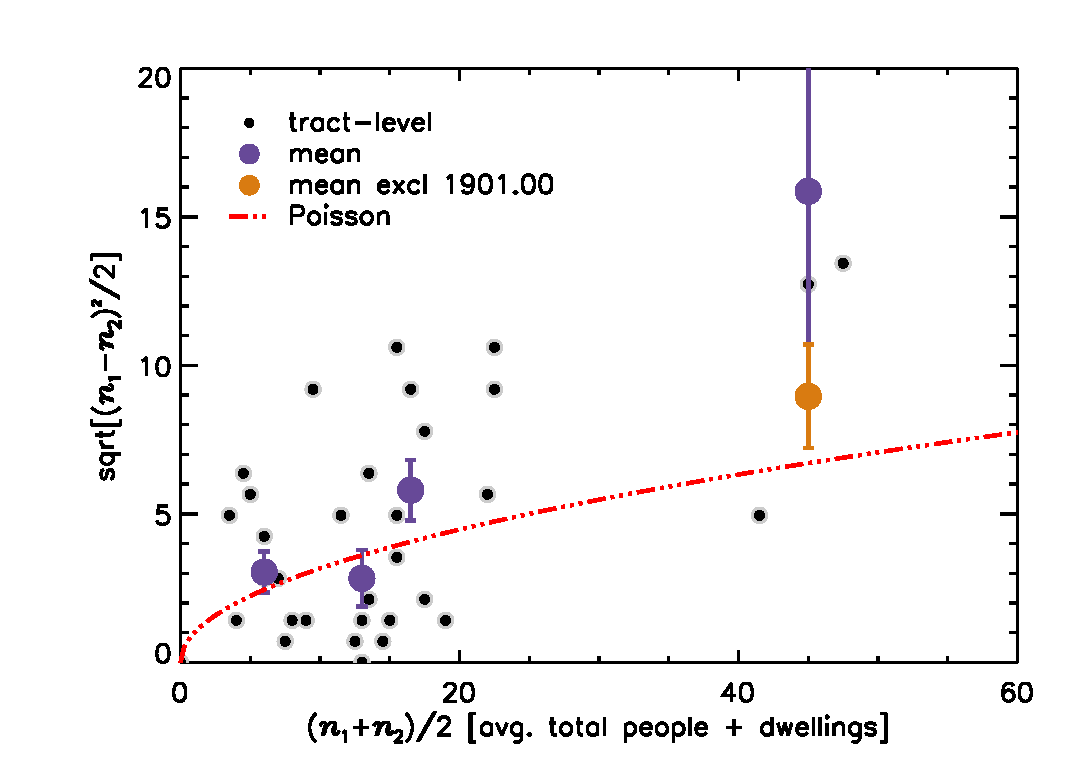
\includegraphics[width=\linewidth]{intDupeChar}\\
	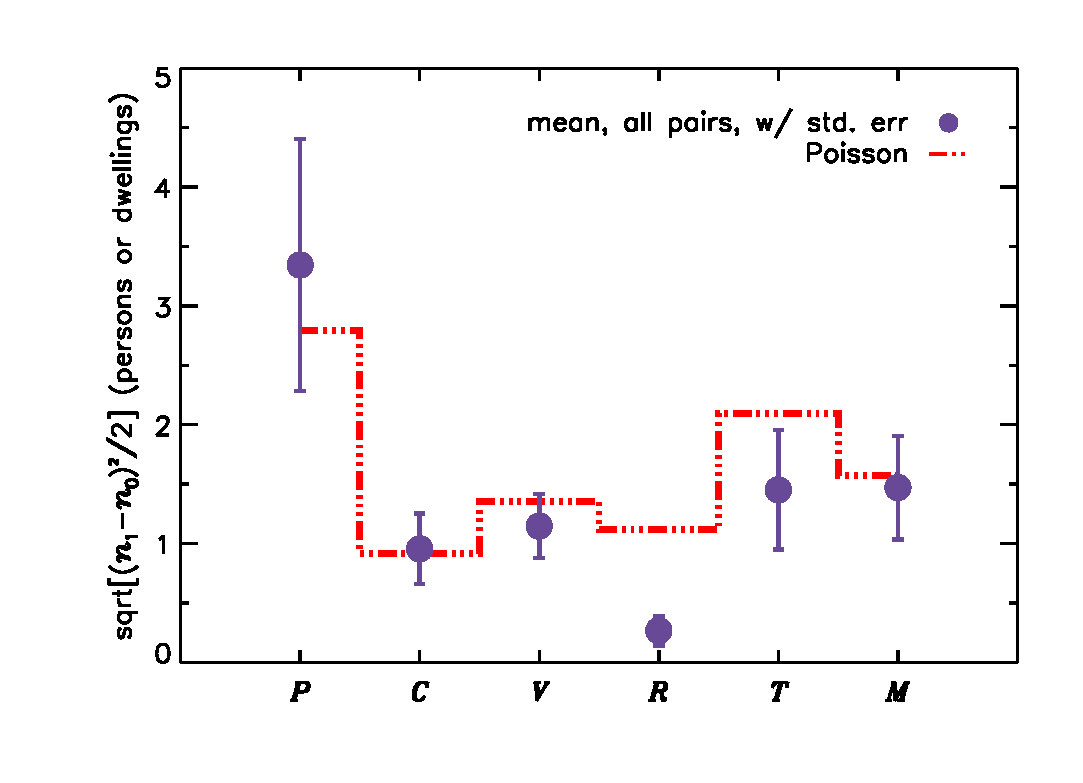
\includegraphics[width=\linewidth]{catDupeChar}
\caption{default}
\label{fig:dupeChar}
\end{figure}

\begin{figure}[]
	\centering
	\includegraphics[width =\linewidth]{volProfComp}
	\caption{}
\end{figure}

Prioritized by raw 2020 counts (Hollywood) or total polulation estimates (EHo). 
Paired by total counts + geography. 
Third pass was first pass with tract pairings presented in reverse order.
\begin{itemize}
	\item All vol tracts counted at least twice;
	\item 4 tracts counted 3x;
	\item One recount DQed for quality flag (1925.20);
	\item Dupe statistics look pretty good. Mean abs discrepancy is consistent
		with zero given standard error on mean except for TAY (2.7 sigma) and RVs (3.8).
		Normalized differences ($|n_{1}-n_{2}|/\sqrt{n_{1}+n_{2}}$) are a little higher
		than $1\sigma$ ($CVRTM=[1.7, 1.1, -, 1.6, 1.4, 0.6, 1.2, 1.6, -]\sigma$), suggesting 
		a little more than poisson counting uncertainty, but LEA cross-checked the one
		highly discrepant ($\sim$8$\sigma$) tract, 1901.00, and found raw counts consistent
		with the average of the two nighttime datasets ($\sim$9:00 AM 26 Feb). 
	\item Above holds true for 1912.01, which is in Hwood and also a SELAH recount tract. LEA
		counted 51 totoal ppl/dwellings 12:30 P on 27 Feb vs 51 by vols night of count.
\end{itemize}

Various governmental, nonprofit, and volunteer organizations\footnote{Including
{\it \href{https://chnc.org}{The Central Hollywood Neighborhood Council}, \href{https://thecenterinhollywood.org}{The Center
at Blessed Sacrament}, \href{https://www.myfriendsplace.org/}{My Friend's Place}, Hang Out Do Good, \href{https://hollywood4wrd.live}
{Hollywood4WRD}}, and various resident organizers.} in Hollywood coordinated a Point-In-Time (PIT) 
enumeration of people experiencing unsheltered homelessness to compensate for the cancellation of the 
official 2021 countywide count. The event took place on 25 February and covered all 39 US Census tracts
in the LAHSA-recognized Hollywood and East Hollywood communities. Nine tracts---mainly along US 
Rte 101---were surveyed by professional outreach teams from {\it The Center at Blessed Sacrament} and
{\it Covenant House} during daylight hours. The remaining 30 tracts were surveyed by 32 car-based volunteer
teams recruited from the local community beginning at 7:00 PM.

Each volunteer team was assigned two tracts in either Hollywood or E.~Hollywood; i.e., no team counted
tracts spanning communities, keeping the two datasets as independent as possible. As such, each tract was
counted by at least two independent teams, with four tracts counted by three teams. This redundancy
enabled assessments of counting uncertainties through inter-counter comparisons, and also increased
accuracy via averaging. The nine professional tracts did not receive duplicate coverage on the day of the 
count, but only one team counted tracts in both Hollywood and E.~Hollywood, largely maintaining the
independence of the two datasets to enable further cross-validation of trends.

In sum, about 20\% of tracts in both communities were counted by professionals. These tracts comprised
roughly 43\% of the total individuals and dwellings counted. Year-on-year trends are consistent between
volunteer- and professionally counted tracts. The largest increase was observed by volunteers, the largest
decrease by professionals; both tracts are located in E.~Hollywood.

{\bfr PRO TRACT RAW COUNT SHARE 2020: 44\% (23 tracts)

PRO TRACT RAW COUNT SHARE 2021: 43\% (all tracts)}

{\bfr Barely consistent if all of last year's vans and cars are still here. 95\% confidence limit $996\pm69$ can reach 1065 (v 1058) 
in Hollywood, $598\pm 59= 657$ vs.\ 656 last yr in E.~Hollywood. BOTH AT 2020 SPA4 WEIGHTS!}


\section{Results}
\label{sec:results}

\begin{table}[]
\caption{Census Tract-level Unsheltered Data}
\resizebox{\linewidth}{!}{%
\begin{tabular}{lcccc}
\toprule
Tract & Team & $n_{\rm teams}$ & Median Est. & 90\% CI \\ 
\cmidrule{1-5}
1898.00 & V & 1 & 8 & 4--14 \\
1899.02 & V & 1 & 23 & 15--32 \\
1899.03 & V & 1 & 3 & 0--8 \\
1899.04 & V & 1 & 38 & 27--50 \\
1899.05 & V & 1 & 20 & 13--29 \\
1901.00 & V & 1 & 67 & 53--80 \\
1902.01 & V & 1 & 36 & 26--47 \\
1902.02 & V & 1 & 23 & 15--31 \\
1903.01 & V & 1 & 109 & 89--131 \\
1905.10 & V & 1 & 52 & 38--66 \\
1907.00 & V & 1 & 106 & 87--124 \\
1908.01 & V & 1 & 88 & 70--105 \\
1908.02 & V & 1 & 88 & 71--106 \\
1909.01 & V & 1 & 39 & 27--52 \\
1909.02 & V & 1 & 26 & 16--36 \\
1910.00 & V & 1 & 156 & 132--181 \\
1917.10 & V & 1 & 12 & 6--19 \\
1917.20 & V & 1 & 25 & 15--35 \\
1918.10 & V & 1 & 45 & 32--58 \\
1918.20 & V & 1 & 16 & 9--23 \\
1919.01 & V & 1 & 58 & 43--73\\
1916.10 & V & 1 & 42 & 28--56 \\
1916.20 & V & 1 & 16 & 9--24
\\ \bottomrule
\end{tabular}
}
\caption*{\bfr this is a placeholder table}
\label{tbl:tractStats}
\end{table}

This section presents CoC level estimates for the number of unsheltered individuals and dwellings
in the Hollywood and East Hollywood areas as of the evening of 25 February 2021. We start with
summaries of each CoC in Sections \ref{sec:hWood} and \ref{sec:eHo} before discussing how these
estimates compare to last year's official LAHSA count in Section \ref{sec:comp}. Section \ref{sec:discussion}
describes how varying elements of Section \ref{sec:mc}'s analysis modulates these results.

\subsection{Hollywood CoC}
\label{sec:hWood}

\begin{figure}[h]
	\centering
	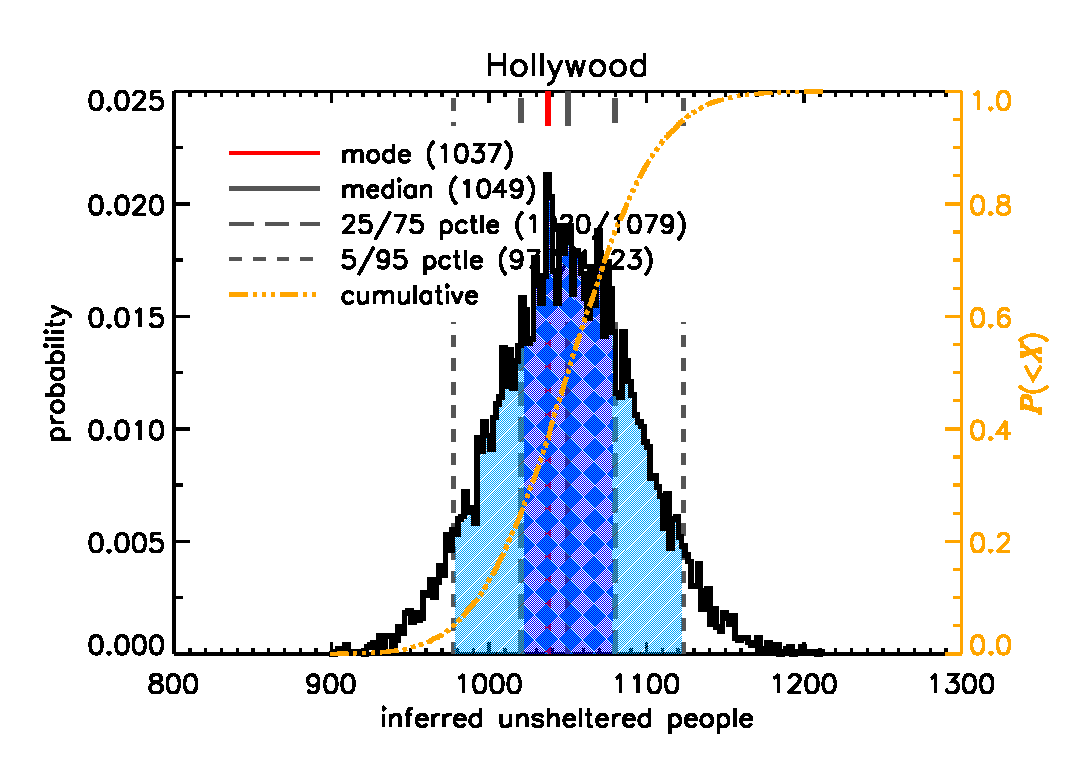
\includegraphics[width =\linewidth]{hWood/HollywoodDist}
	\caption{}
\end{figure}

\subsection{East Hollywood CoC}
\label{sec:eHo}

\begin{figure}[h]
	\centering
	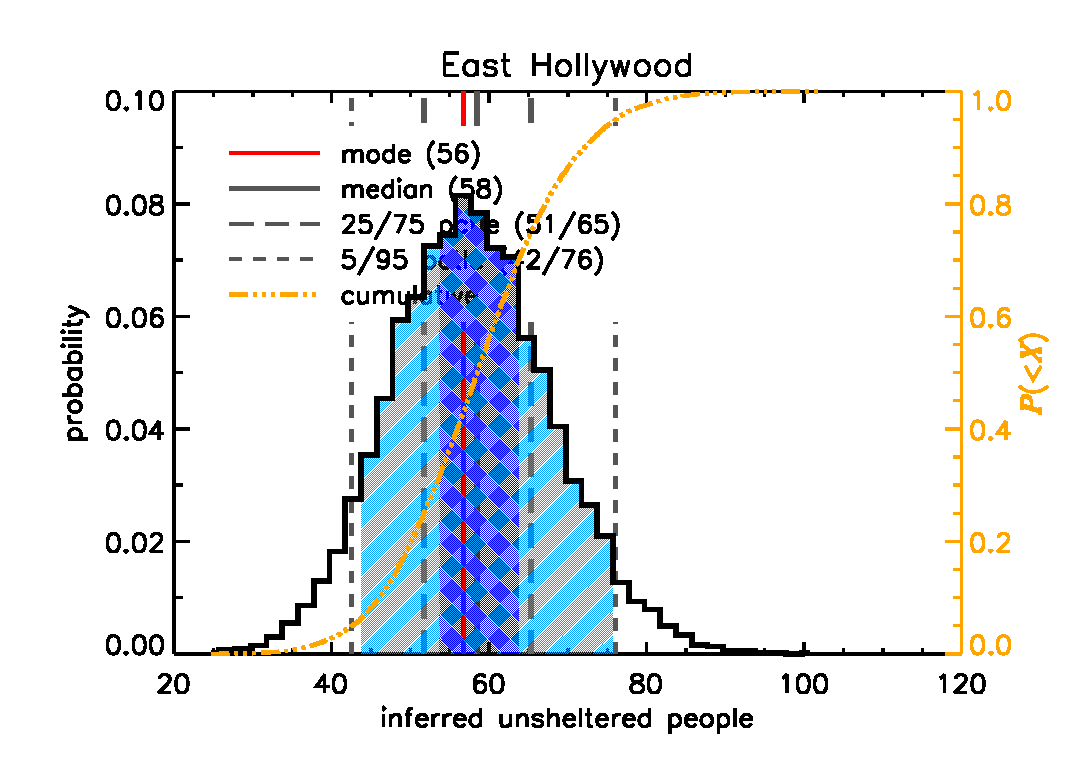
\includegraphics[width =\linewidth]{eHo/EastHollywoodDist}
	\caption{}
\end{figure}

\begin{figure*}[h]
	\centering
	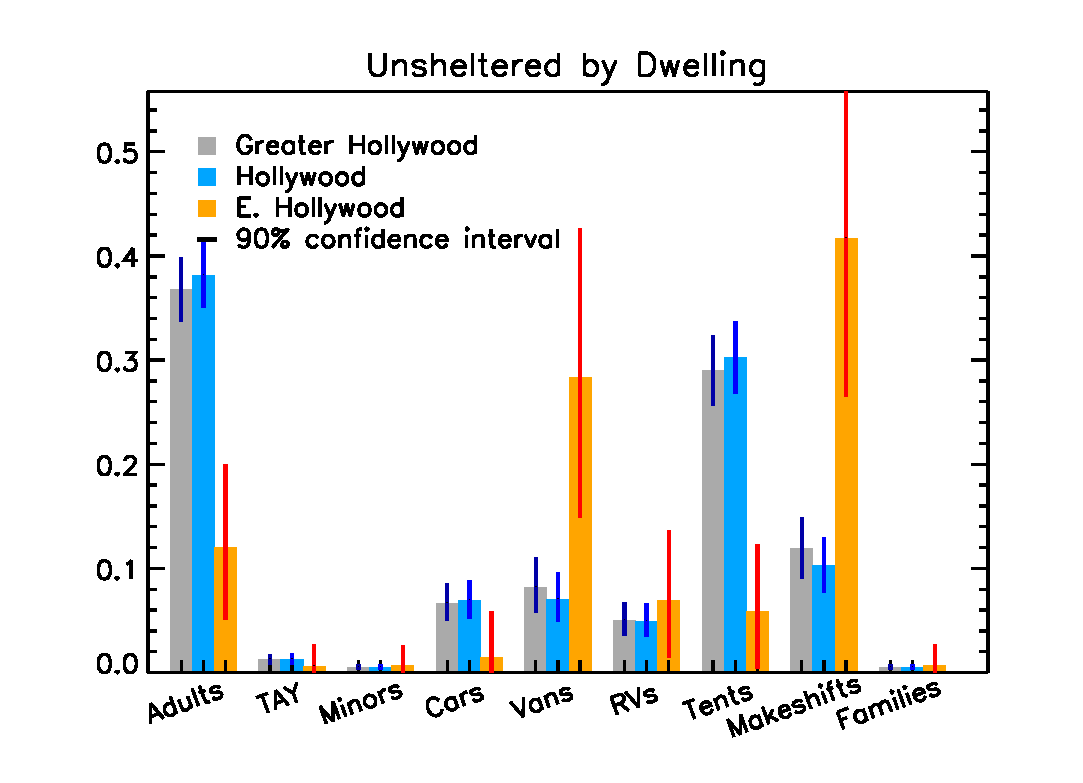
\includegraphics[width =\linewidth]{allTracts/allBreakdownBar}
	\caption{}
\end{figure*}

\subsection{Comparison to 2020}
\label{sec:comp}

\section{Systematics}
\label{sec:systematics}

We discuss these potential sources of systematic errors below.

\subsection{Null Entries}
\label{sec:nulls}

As stated in Section \ref{sec:training}, some (too few) tracts have unsheltered populations near zero, 
or at least are not observed to host any people or dwellings of a specific category. Such null entries 
are consistent with a range of non-zero values for the true population due to shot noise. As such, the 
Monte Carlo PDF reconstruction must allow them to take non-zero values based on an assumed background
rate. 
%This fact is immaterial 
%when the global category population is high, but such is not the case for TAY, unaccompanied 
%minors, and families. Treatment of null entries therefore affects estimates for those sub-populations,
%or defines their upper limits.

Ideally, that rate would be based on the variations in a category's counts (or count densities) in other, 
similar tracts defined by some independent criteria. While sufficient data from, e.g., the US Census 
may enable such an exercise, it is beyond the scope of this analysis. Instead, we base our noise floor 
on the number of counts of a given category expected if the total was evenly distributed across 
all tracts. That is:
\begin{equation}
	\sigma_{j,\,\rm min}^{2} = \frac{1}{39}\sum_{\rm tracts}n_{j},
\end{equation}
where $\sigma_{j}$ and $n_{j}$ are defined as in Equation \ref{eq:monte}.

This method works for any category, $j$, for which there is at least one individual/dwelling observed in any 
tract. However, for categories for which even this is not the case---unaccompanied minors and families, in the
case of Hollywood---we set $\sigma_{j, \rm min}$ to the lowest non-zero value of the other categories
(corresponding to TAY).

{\bfr State the bkg levels.}

{\it While we admit that such a treatment is 
somewhat arbitrary}, due to the intrinsically low levels of at least unsheltered unaccompanied minors 
and families, it does not significantly affect our CoC level estimates. It does affect TAY, however, and
as such, taken with the difficulty of disambiguating older TAY from younger adults, we caution against 
relying on the TAY estimates for anything beyond lower-limits.

\subsection{CVRTM Biases}
\label{sec:CVRTM}

\begin{figure*}[h!]
	\centering
	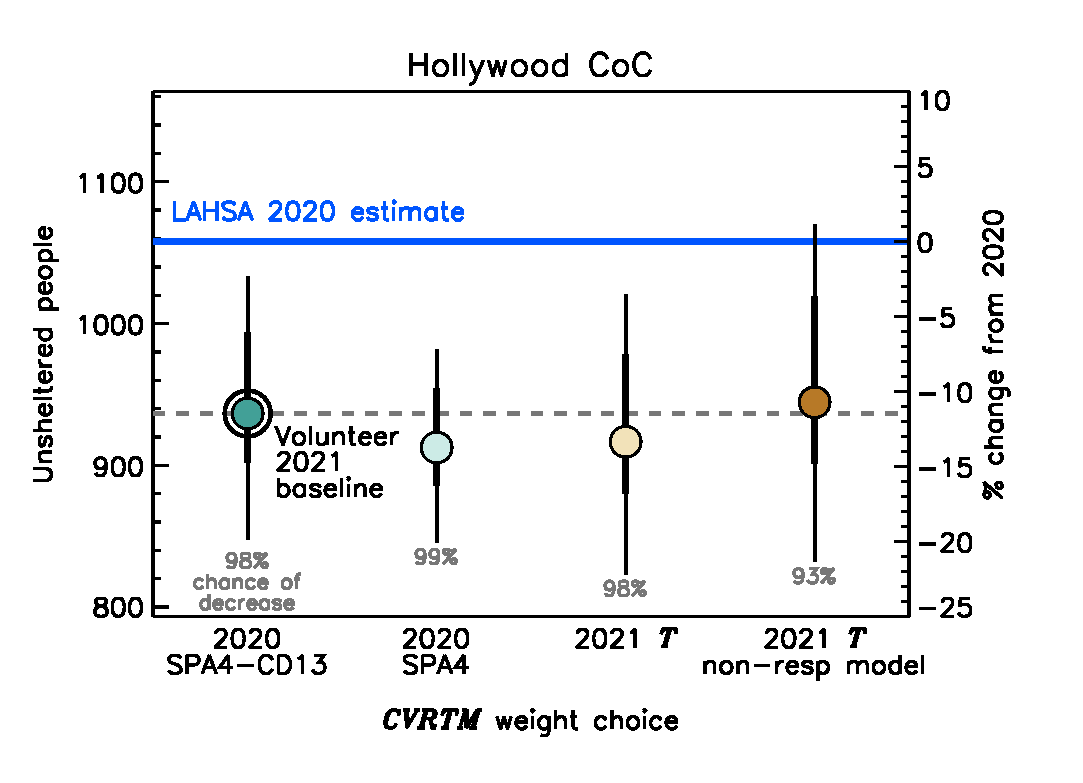
\includegraphics[width = 0.48\textwidth, trim = 0cm 0.5cm 0cm 0cm]{hwoodFinal}
	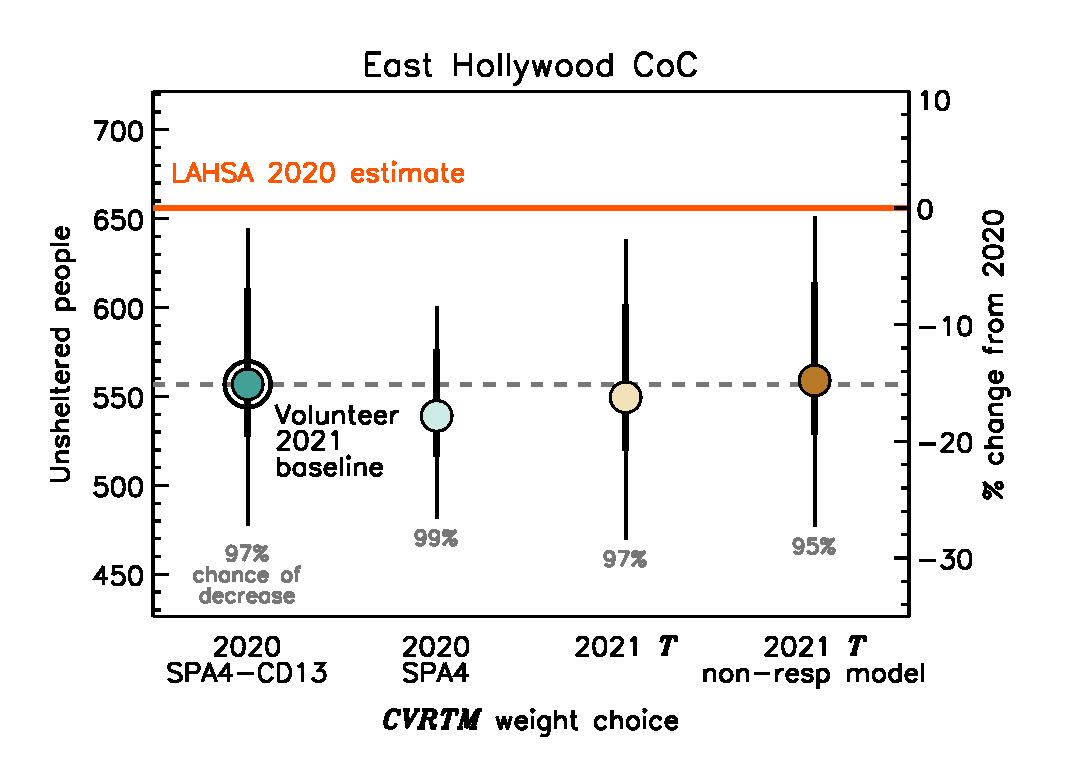
\includegraphics[width = 0.48\textwidth, trim = 0cm 0.5cm 0cm 0cm]{ehoFinal}	
	\caption{Unsheltered populations in Hollywood (left) and East Hollywood (right) 
			as functions of CVRTM weights. The baseline estimate uses the same weights as the 
			2020 LAHSA Community Summaries. Using SPA4 weights or replacing the tent 
			weight, $T$, with results from a survey conducted in Hollywood yields consistent
			results. All imply at least a 93\% chance that unsheltered homelessness has fallen
			by some amount, with likely declines of $12\%\pm9\%$ and $15\%\pm12\%$
			in Hollywood and East Hollywood, \resp.}
	\label{fig:wtComp}
\end{figure*}

\begin{table*}[h!]
\caption{Greater Hollywood 2021 PIT Unsheltered Data and Population Estimates}
\resizebox{\linewidth}{!}{%
\begin{tabular}{lcccccccccc}
\toprule
 & Adult & TAY & Car & Van & RV & Tent & Makeshift & {\bf 2021 Total} & {\bf 2020 Total} & {\bf Difference} \\ \cmidrule{1-11}
{\bf Hollywood} \\ %\cmidrule{1-1}
Counts & 277 & 2 & 21 & 27 & 34 & 224 & 115 & {\bf 702} & {\bf 831} & $\bf -15\%$ \\
Inhabitants & 277 (27) & 2 (5) & 32 (11) & 49 (13) & 50 (14) & 332 (29) & 195 (24) & {\bf 937 (93)} & {\bf 1058} & $\bf -11\%\,(9\%)$\\% (76)
Category share & 30\% (3\%) & 0\% (0\%) & 3\% (1\%) & 5\% (1\%) & 5\% (1\%) & 35\% (3\%) & 21\% (3\%) & -- & -- & -- \\ \cmidrule{1-11}
{\bf East Hollywood} \\ %\cmidrule{1-1}
Counts & 114 & 4 & 10 & 39 & 16 & 77 & 127 & {\bf 389} & {\bf 469} & $\bf -17\%$ \\
Inhabitants & 114 (19) & 4 (4) & 15 (8) & 70 (15) & 24 (9) & 115 (19) & 216 (23) & {\bf 557 (83)} & {\bf 656} & $\bf -15\%\,(12\%)$\\% (60)
Category share & 20\% (3\%) & 1\% (1\%) & 3\% (1\%) & 13\% (3\%) & 4\% (2\%) & 20\% (3\%) & 39\% (4\%) & -- & -- &--
\\ \bottomrule
\end{tabular}
}
\caption*{Parentheses denote 90\% uncertainties(binomial in the case of the categories). 
Uncertainties larger than estimates imply that only upper limits are available. No unaccompanied 
minors or families were observed.}
\label{tbl:summary}
\end{table*}

Less easily handled are potential biases in the CVRTM demographic weights our \Count\ adopts.
Typically, specialized teams perform detailed interviews of people experiencing homelessness to update 
these weights in various geographic contexts. However, the cancellation of the official PIT count means
that this will not occur in 2021. As such, we are forced to rely on year-old estimates.

We present 

\begin{figure*}[h]
	\centering
	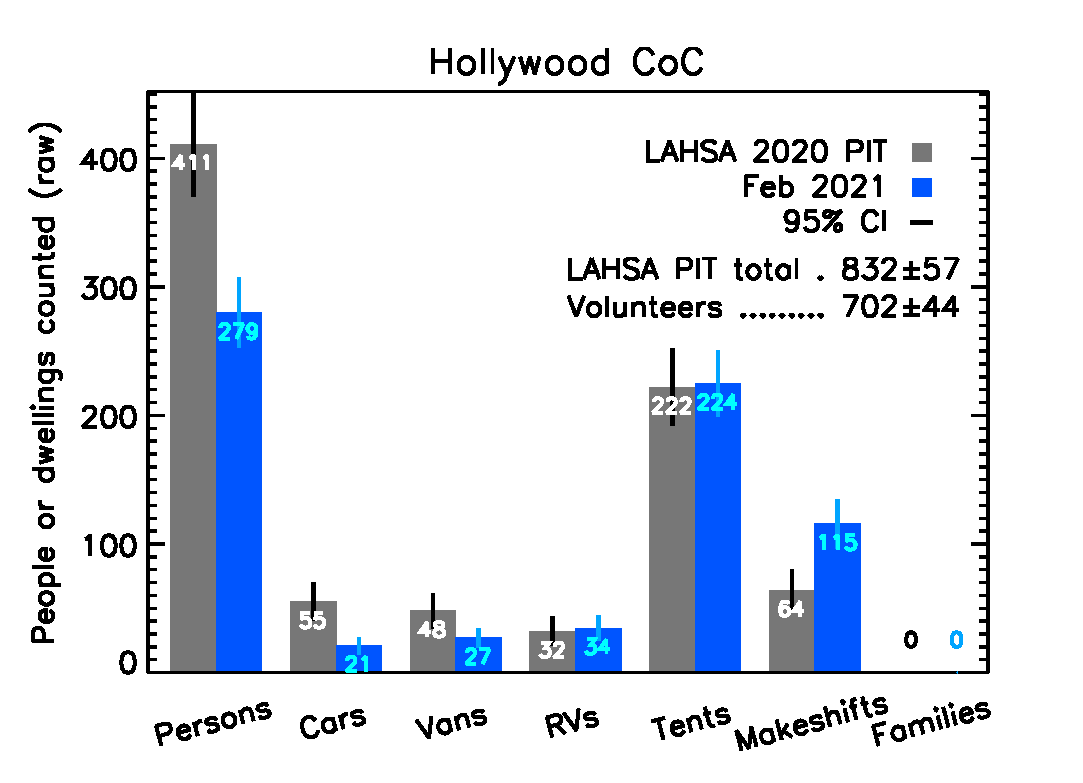
\includegraphics[width = 0.47\textwidth, trim = 1cm 0cm 0cm 0cm]{Hwood2021Bars}
	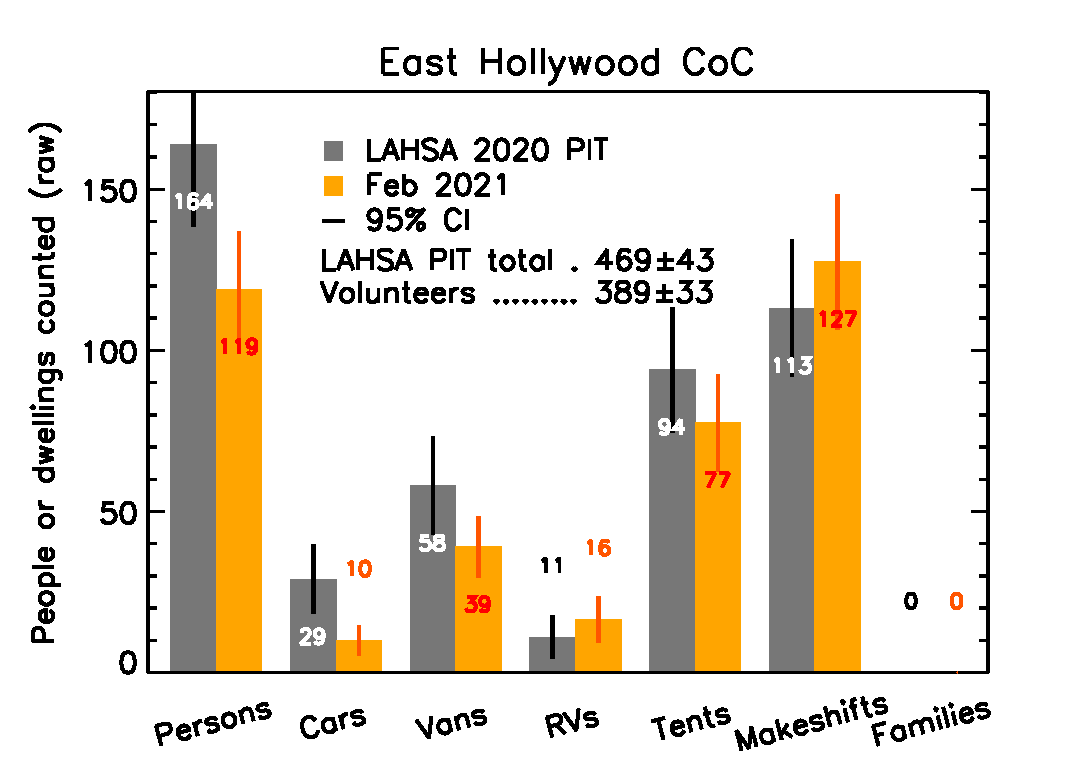
\includegraphics[width = 0.47\textwidth, trim = 0cm 0cm 1cm 0cm]{Eho2021Bars}
	\caption{Raw tallies of unsheltered persons and dwellings in Hollywood and East Hollywood
			(left/right) from the 2020 and 2021 PIT counts (grey/colors). Persons, cars, 
			and vans fell in both communities while RVs and tents stayed statistically flat. 
			Makeshift structures are the only category to show a potential common increase. 
			Overall, we identified 208 fewer people and dwellings compared to 2020,
			with similar 16\% decreases assessed by almost entirely independent teams
			in both communities. ``Persons'' are TAY+Adults.}
	\label{fig:rawCounts}
\end{figure*}

\begin{figure}[]
	\centering
	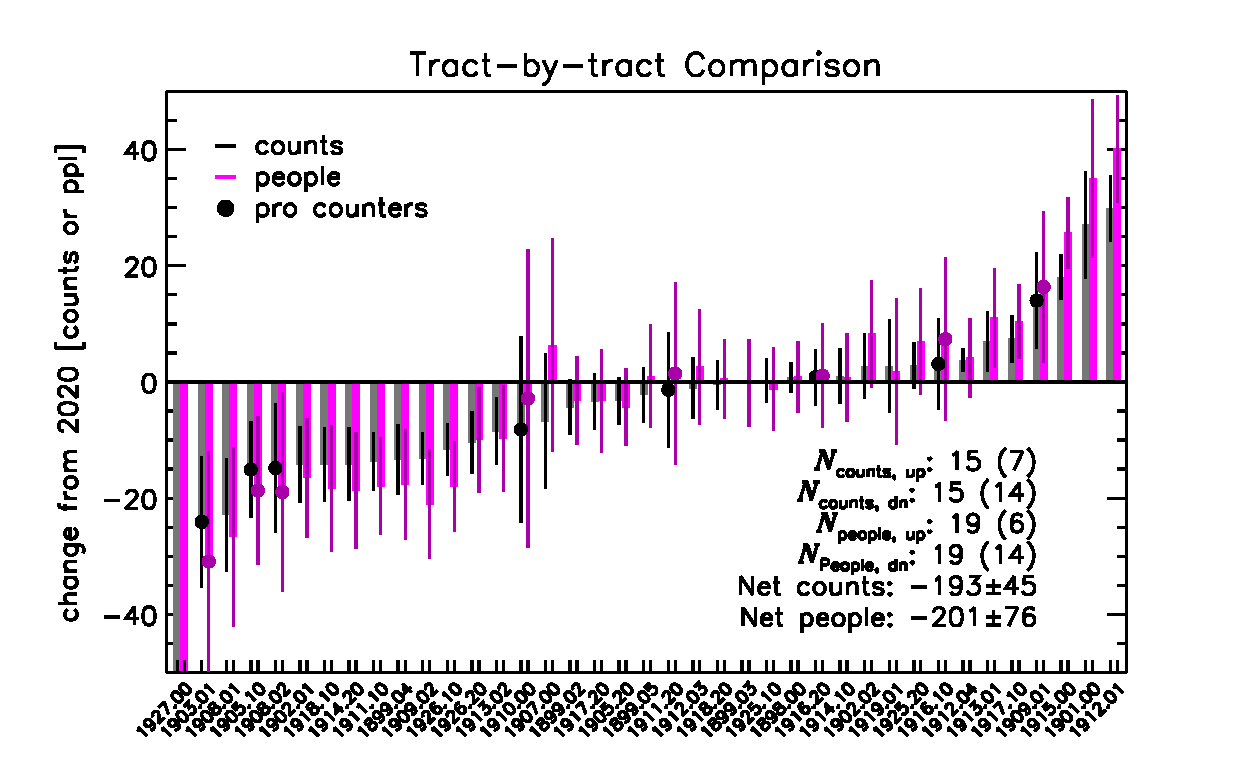
\includegraphics[width = \textwidth, trim = 0cm 0cm 0cm 0cm]{tractsYrYr}
	\caption{}
	\label{fig:tractYrYr}
\end{figure}

\subsubsection{Nulling the 2021 Result}
\label{sec:nullOut}

\subsubsection{Examining Past Variability}
\label{sec:pastValues}

\subsubsection{Relying on Smaller Geographies}
\label{sec:cdWts}

\subsubsection{Using External Data}
\label{sec:bidData}

The Hollywood Partnership---one of Hollywood's Business Improvement Districts (BIDs)---has performed
weekly visual scans of its footprint since spring 2019. These inspections tally unsheltered people and 
tents separately. As such, they can be used to bound the possible evolution of the CVRTM tent weight
between the official 2020 value and what it may be today.

{\bfr SECZ}

A lower-bound on the the weight can be derived by assuming that all of the tents captured by the BID's 
censuses were empty and all of their inhabitants visible. The weight would the be just the number of
people on the number of tents. If any of the tents were not empty, the true weight would be higher than
the inferred weight. Ergo, the BID/SECZ derived tent weight may reflect a {\it conservative} estimate 
which, when applied to the entire footprint, would produce something like a lower-bound on the 
tent contribution to the 2021 \Count.

{\bfr We'll use the BID counts outside the SEZ and find (tents+people)/tents for the past year. We'll
fit it and get a range of values for the night of the count. It's typically higher than 1.45 (thru last July,
at least), so we can just find the decline and peg it to 1.45.}

{\bfr Plot the trend; discuss it in terms of the 2020 value; see what it does; talk about why we don't
think most of the folks on foot in the SECZ are interlopers.}

\section{Discussion}
\label{sec:discussion}

\begin{figure}[]
	\centering
	\includegraphics[width =\linewidth]{tract1907comp}
	\caption{}
\end{figure}

PRK effects.

ABH effects.

PSH effects.

{\bfr 1907.00 people and tents switched. Total unsheltered $\sim$constant but visual perceptions
in this most-highly trafficked tract will make it *feel* like homelessness has increased by a lot.}

SPLA.

Edges.

\section{Summary}
\label{sec:summary}

\section*{}

{\bfr Acknowledge Kelson}

\appendix

\section{Example Documents}

\begin{figure*}
	\centering
	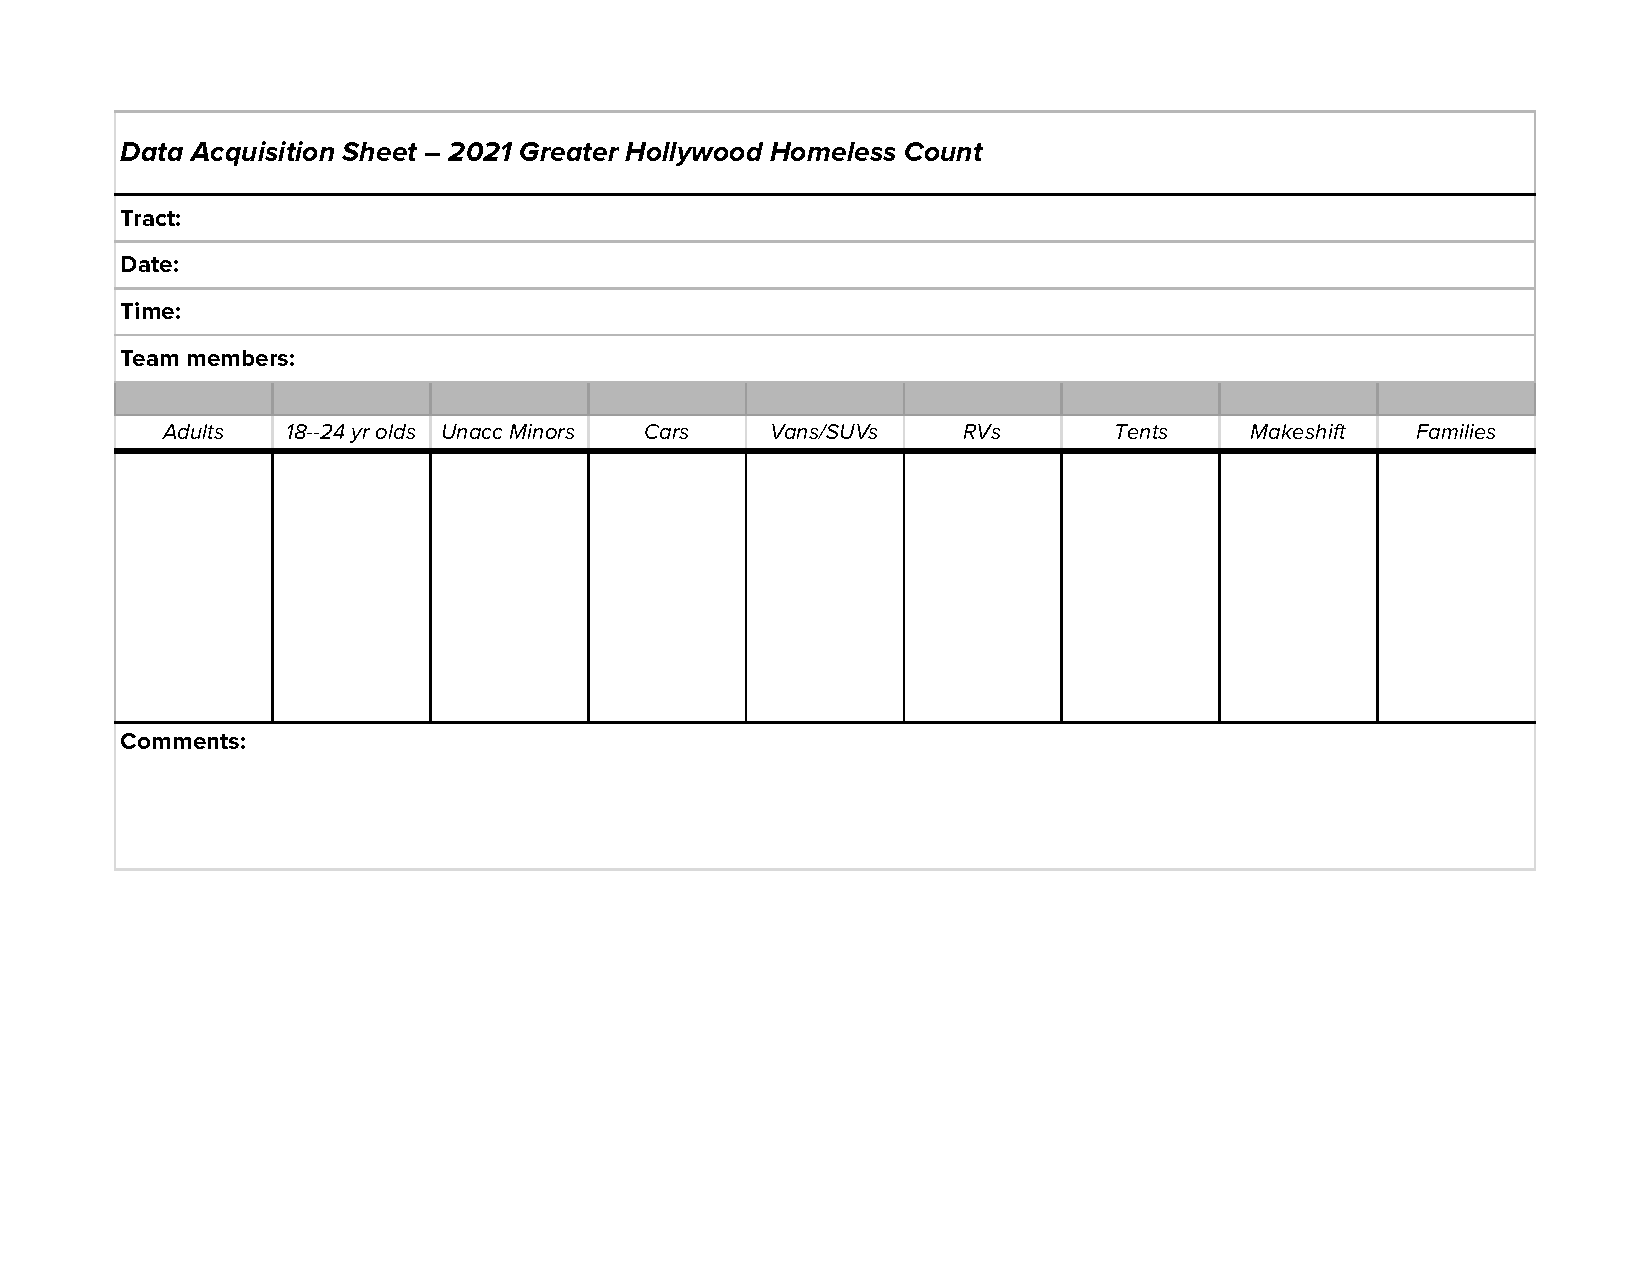
\includegraphics[width =\linewidth]{Hollywood2021CountDataSheet}
	\caption{Counter tally-sheet}
\end{figure*}

\begin{figure*}
	\centering
	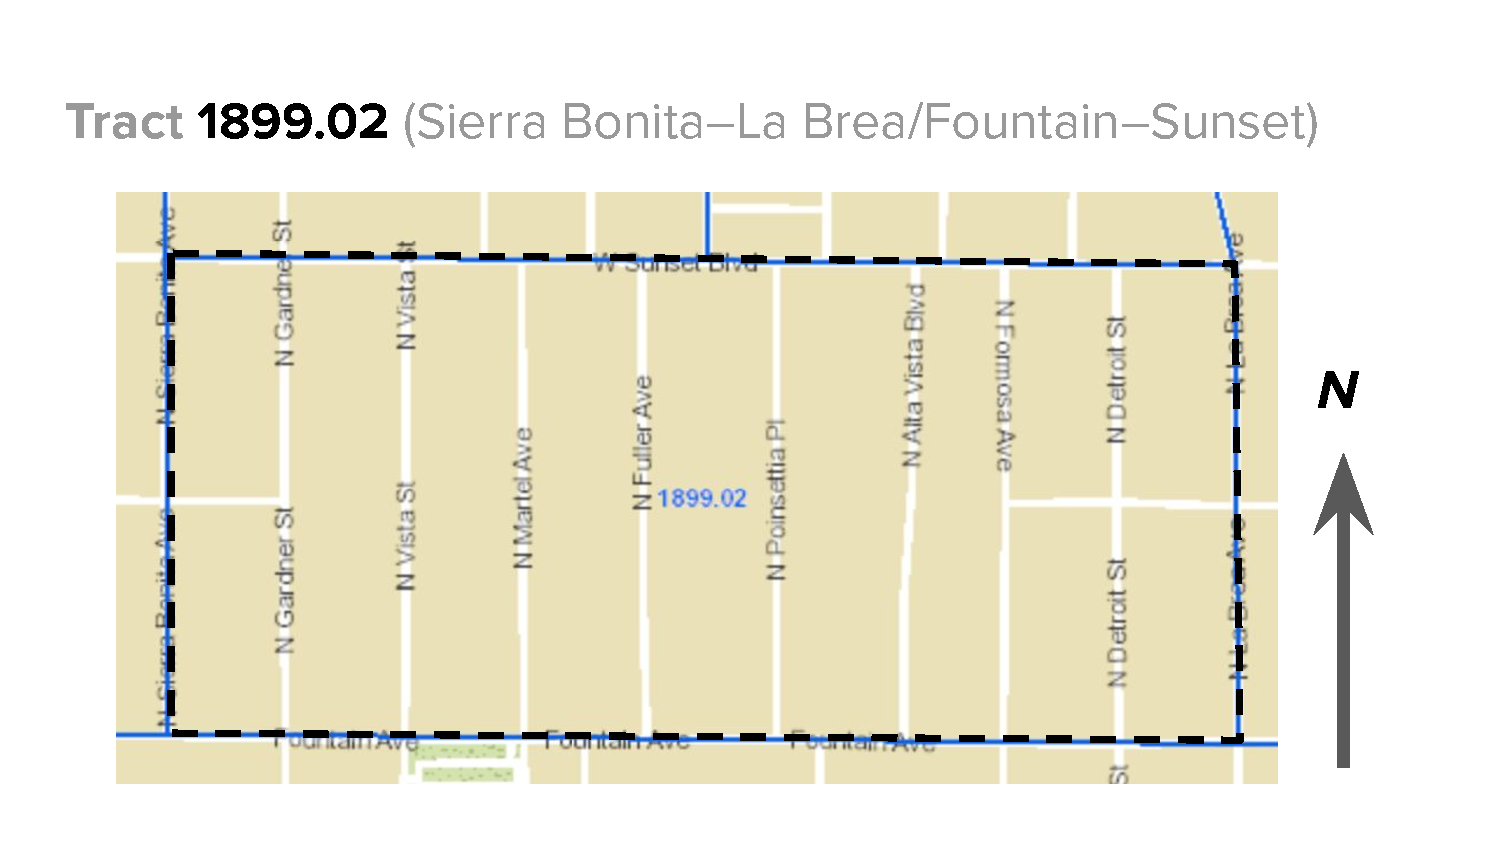
\includegraphics[width =\linewidth]{tractMap}
	\caption{Example Hollywood tract map.}
\end{figure*}

\begin{figure*}
	\centering
	\includegraphics[width =0.7\linewidth]{primerFront}
	\caption{Count primer {\bfr SCRUB EK'S NUMBER!}}
\end{figure*}

\section{Full Tract-level Results}


\begin{table*}[]
\caption{Tract 1898.00 Unsheltered Data}
\resizebox{\linewidth}{!}{%
\begin{tabular}{lcccccccccc}
\toprule
 & Adult & TAY & Unacc Minor & Car & Van & RV & Tent & Makeshift & Family & {\bf Total} \\ \cmidrule{1-11}
Counts & 3 & 0 & 0 & 0 & 0 & 0 & 1 & 1 & 0 & {\bf 5} \\
Inhabitants & 3 (3) & 0 (1) & 0 (1) & 1 (2) & 1 (2) & 1 (2) & 2 (2) & 2 (2) & 0 (1) & {\bf 9 (6)} \\
Category share & 0.31 (0.29) & 0.03 (0.10) & 0.03 (0.10) & 0.09 (0.18) & 0.10 (0.19) & 0.07 (0.16) & 0.16 (0.23) & 0.18 (0.24) & 0.03 (0.10) & - 
\\ \bottomrule
\end{tabular}
}
\caption*{Quantities in parentheses denote 95\% uncertainties (binomial in the case of the categories). Uncertainties larger than estimates imply that only upper limits can be stated confidently.}
\label{tbl:}
\end{table*}

\end{document}  